\section{Машинное обучение} \label{ML}

\subsection{Понятие искусственной нейронной сети}

Машинное обучение – раздел исследований в сфере ИИ, в основе которых лежат методы разработки систем способных к обучению. Алгоритмы машинного обучения эффективно себя показывают в задачах, в которых требуется у заранее подготовленных (обучающих) данных определить общие признаки и по ним идентифицировать новые данные. В проектировании таких, обучающихся, систем часто применяют искуственные нейронные сети. 

Искусственная нейронная сеть (ИНС) – компьютерная модель, в основе которой лежат принципы работы биологической нейронной сети - совокупности связанных между собой нервных клеток - нейронов. Каждый нейрон имеет набор входных связей - синапсов, по которым он получает информацию, представленную в виде импульсов, от других нейронов. По полученным данным нейрон формирует своё состояние и, с помощью аксона, сообщает его другим нейронам, обеспечивая функционирование системы. В процессе формирования системы одни нейронные связи укрепляются, а другие ослабляются, обеспечивая обучаемость сети.
\addimghere{biological-neuron}{0.5}{Типичная структура биологического нейрона}{biological-neuron}

Искусственный нейрон представляет собой упрощенную модель биологического нейрона. Принцип его работы представлен на рисунке \ref{simple-neuron}. Сначала нейрон получает n-мерные вектор входных значений $X=(x_{1},...,x_{n})$ и вектор весов $W=(w_{1},...,w_{n})$, обозначающий <<укрепленность>> межнейронных связей. Вычисляется сумма произведений входных значений и весов $s_j$. Затем к полученному результату применяется \hyperref[sec:activation]{функция активации} $\varphi$. Дополнительно, к сумме может прибавляться величина смещения $b_j$.
\begin{figure}[H]
  \centering

  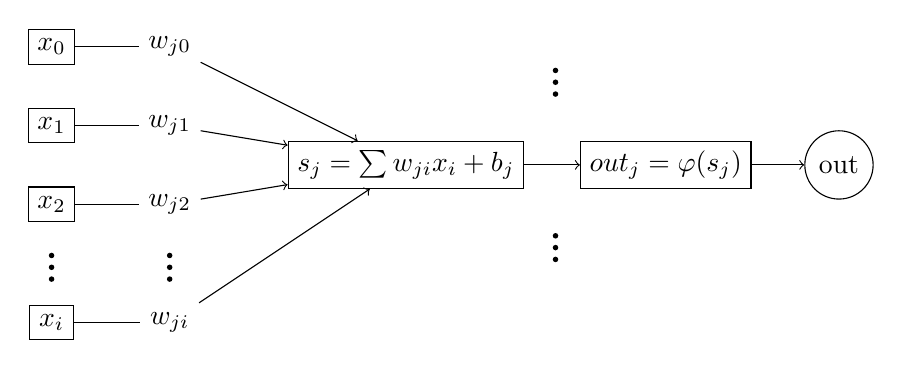
\begin{tikzpicture}
    \tikzstyle{rectangle_style}=[rectangle, draw]
    \tikzstyle{dividedrectangle_style}=[draw, rectangle split, rectangle split parts=2, rotate = 90, minimum height = 15mm, minimum width = 10mm]
    
    % neuron i
    \foreach \x in {0,...,2}
      \draw node at (0, -\x) [rectangle_style] (neuron_i_\x) {$x_\x$};
    \foreach \x in {1,...,3}
      \fill (0, -2.5 - \x*0.15) circle (1pt);
    \draw node at (0, -3.5) [rectangle_style] (neuron_i_3) {$x_i$};
    
    % w_ji
    \foreach \x in {0,...,2}
      \draw node at (1.5, -\x) [] (w_ji_\x) {$w_{j\x}$};
    \draw node at (1.5, -3.5) [] (w_ji_i) {$w_{ji}$};
    \foreach \x in {1,...,3}
      \fill (1.5, -2.5 - \x*0.15) circle (1pt);
    
    % neuron sum
    \draw node at (4.5, -1.5) [rectangle_style] (neuron_sum) {
      $s_j = \sum {w_{ji}x_i+b_j}$
    };
    \draw node at (7.8, -1.5) [rectangle_style] (neuron_act) {
      $out_j = \varphi (s_j)$
    };
    \foreach \x in {1,...,3}
      \fill (6.4, -2.25 - \x*0.15) circle (1pt);
    \foreach \x in {1,...,3}
      \fill (6.4,  - 0.15 - \x*0.15) circle (1pt);
    
    % output
    \node at (10, -1.5) [circle, draw] (output) {out};    

    
    % connect: y_i -> w_ji
    \foreach \i in {0,...,2}
      \path[-] (neuron_i_\i) edge node[] {} (w_ji_\i);
    \path[-] (neuron_i_3) edge node[] {} (w_ji_i);
    
    % connect: w_ji -> neuron j
    \foreach \i in {0,...,2}
      \path[->] (w_ji_\i) edge node[] {} (neuron_sum);
    \path[->] (w_ji_i) edge node[] {} (neuron_sum);
    
     % connect: neuron sum  -> neuron act
     \path[->] (neuron_sum) edge node[above, midway] {$ $} (neuron_act);

    % connect: neuron act -> output
    \path[->] (neuron_act) edge node[above, midway] {$ $} (output);

    
  \end{tikzpicture}
\caption{Схема искусственного нейрона} \label{simple-neuron}
\end{figure}

Множества нейронов формируют слои. Слои в свою очередь формируют нейронную сеть. Входной слой получает данные, обрабатывает и передает нейронам скрытого слоя. Аналогично срабатывает каждый последующий слой вплоть до выходного. 

\tikzset{%
every neuron/.style={
  circle,
  draw,
  minimum size=1cm
},
neuron missing/.style={
  draw=none, 
  scale=4,
  text height=0.333cm,
  execute at begin node=\color{black}$\vdots$
},
}
\begin{figure}[H]
  \centering
\begin{tikzpicture}[x=1.5cm, y=1.5cm, >=stealth]

\foreach \m/\l [count=\y] in {1,2,3,missing,4}
\node [every neuron/.try, neuron \m/.try] (input-\m) at (0,2.5-\y) {};

\foreach \m [count=\y] in {1,missing,2}
\node [every neuron/.try, neuron \m/.try ] (hidden-\m) at (2,2-\y*1.25) {};

\foreach \m [count=\y] in {1,missing,2}
\node [every neuron/.try, neuron \m/.try ] (output-\m) at (4,1.5-\y) {};

\foreach \l [count=\i] in {1,2,3,n}
\draw [<-] (input-\i) -- ++(-1,0)
  node [above, midway] {$I_\l$};

\foreach \l [count=\i] in {1,k}
\node [above] at (hidden-\i.north) {$H_\l$};

\foreach \l [count=\i] in {1,p}
\draw [->] (output-\i) -- ++(1,0)
  node [above, midway] {$O_\l$};

\foreach \i in {1,...,4}
\foreach \j in {1,...,2}
  \draw [->] (input-\i) -- (hidden-\j);

\foreach \i in {1,...,2}
\foreach \j in {1,...,2}
  \draw [->] (hidden-\i) -- (output-\j);

\foreach \l [count=\x from 0] in {Входной, Скрытый, Выходной}
\node [align=center, above] at (\x*2,2) {\l \\ слой};
\end{tikzpicture}
\caption{Схема простой нейронной сети} \label{simple-network}
\end{figure}

Нейросети с большим количеством скрытых слоев называется глубокими. Область машинного обучения, в которой используются глубокие нейронные сети называется глубоким обучением.     

\subsection{Активационная функция}
\label{sec:activation}
Взвешенная сумма входов представляет собой линейную комбинацию, из чего следует, что независимо от количества слоев, значения выходного слоя зависят только от входов первого слоя. 
Активационная функция нейрона обеспечивает нормализацию посчитанной суммы и нелинейность нейронной сети. Для многих моделей нейронных сетей также требуется, чтобы активационная функция была монотонной и непрерывно-дифференцируемой на всей области определения.

Существует большое количество функций активации. Наиболее распространенные из них представлены в таблице \ref{actvs}.

\pgfplotsset{
  every axis plot/.append style={
    line width=3pt
  }
}

\begin{table}[H]
  \centering
  \caption{Популярные активационные функции}\label{actvs}
  \begin{tabular}{|c|c|c|}
    \hline    
    \hyperlink{name}{Название} & \hyperlink{func}{Функция} & \hyperlink{chart}{Вид}\\
    \hline
    Сигмоидная &  \resizebox{0.2\hsize}{!}{$\sigma(x)=\frac{1}{1+e^{-x}}$}
    & 
    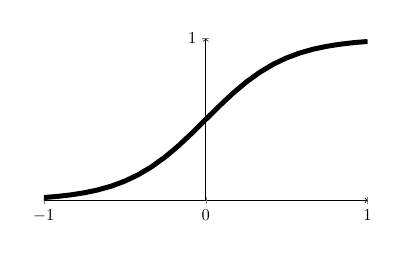
\begin{tikzpicture}[baseline={(0,0.8)}, scale=0.6]      
      \begin{axis}[
        axis equal image,
        axis lines=middle,
        axis line style={->},
        x label style={at={(axis description cs:0.5,-0.1)},anchor=north},
        y label style={at={(axis description cs:-0.1,.5)},rotate=90,      anchor=south},
        extra x ticks=0,
        % extra y ticks=1,
        ymin=0,ymax=1,
        ytick={0, 1},
        xtick={-1, 0, 1}
        ]
        \addplot[domain=-1:1, variable=\x] ({\x},{1/(1+exp(-4*\x))});
      \end{axis}      
    \end{tikzpicture}
   
    \\
    \hline
    Гиперболический тангенс 
    &
    \resizebox{0.2\hsize}{!}{$f(x)=\frac{e^x-e^{-x}}{e^x+e^{-x}}$}
    & 
    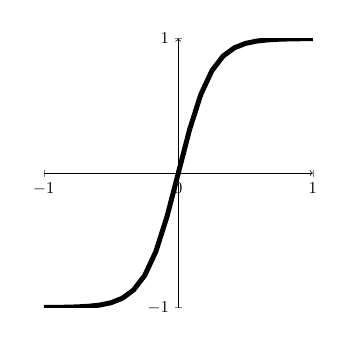
\begin{tikzpicture}[baseline={(0,1.5)},scale=0.6]
      \begin{axis}[
        axis equal image,
        axis lines=middle,
        axis line style={->},
        x label style={at={(axis description cs:0.5,-0.1)},anchor=north},
        y label style={at={(axis description cs:-0.1,.5)},rotate=90,      anchor=south},
         extra x ticks=0,  
        % extra y ticks=1,
        ymin=-1,ymax=1,
        ytick={-1, 0, 1},
        xtick={-1, 0, 1}
        ]
        \addplot[domain=-1:1, variable=\x]({\x},{tanh(4*\x)});
      \end{axis}      
    \end{tikzpicture} 
    \\
    \hline
    ReLU & \resizebox{0.2\hsize}{!}{$f(x) =\begin{cases}
    0, & x<0 \\ 
    x, & x \geq 0.
    \end{cases}$} & 
    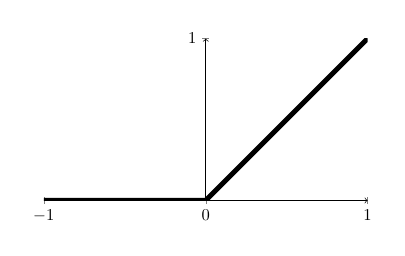
\begin{tikzpicture}[baseline={(0,0.8)},scale=0.6]
      \begin{axis}[
        axis equal image,
        axis lines=middle,
        axis line style={->},
        x label style={at={(axis description cs:0.5,-0.1)},anchor=north},
        y label style={at={(axis description cs:-0.1,.5)},rotate=90,anchor=south},
         extra x ticks=0,  
        % extra y ticks=1,
        ymin=0,ymax=1,
        ytick={0, 1},
        xtick={-1, 0, 1}
        ]
        \addplot[domain=-1:1, variable=\x]({\x},{ifthenelse(\x<0,0,\x)});
      \end{axis}      
    \end{tikzpicture}
    \\
    \hline
  \end{tabular}
\end{table}

Отдельно стоит упомянуть функцию Softmax. Эта функция часто применяется на последнем слое глубоких нейронных сетей в задачах классификации. Пусть последний слой сети содержит N нейронов, каждый из которых соответствует некоторому классу. Тогда значение выхода i-го нейрона вычисляется по формуле: 
\[
    y_i=\frac{e^{z_i}}{\sum\limits_{j=1}^{N}e^{z_j}}
\]
Таким образом, результат каждого нейрона будет принимать значения из диапазона $[0,1]$, а их сумма равна 1. По итогу, сеть выдаст вероятности отношения входных данных к заданным классам.
\clearpage
\subsection{Обучение нейронных сетей}
Под обучением нейронных сетей подразумевается подбор значений весов связей для эффективного решения поставленной задачи. Изначально, веса устанавливаются случайно. Затем, в процессе прогона через сеть тестовых данных, веса корректируются так, чтобы в конечном итоге сеть выдавала правильные ответы. 

Процесс обучения проходит циклично. За одну итерацию на сеть подается пакет, содержащий некоторое количество элементов из входных данных. Разовый проход через сеть всего набора тестовых данных называется эпохой.

Для того, чтобы контролировать процесс обучения необходимо как-то оценивать работу сети. Для этого вводится функция потерь (функция стоимости), которая вычисляет разницу между правильными и полученными результатами и формирует некоторое численное значение, характеризующее величину ошибки работы сети. Таким образом задача обучения сети сводится к задаче поиске глобального минимума данной функции. В таблице \ref{loss_funcs} указаны наиболее часто используемые функции потерь, где $y_i$ – ожидаемое значение i-го нейрона, $x_i$ – полученное значение i-го нейрона, n – количество выходных нейронов.

 \pgfplotsset{
  every axis plot/.append style={
    line width=3pt
  }
}

\begin{table}[H]
  \centering
  \caption{Популярные функции потерь} \label{loss_funcs}
  \begin{tabular}{|c|c|}
    \hline    
    \hyperlink{name}{Название} & \hyperlink{func}{Функция}\\
    \hline
    Средняя квадратическая ошибка & $E=\frac{1}{N}\displaystyle\sum\limits_{i=1}^{n}(y_i - x_i)^2$\\
    \hline
    Средняя абсолютная ошибка & $E=\frac{1}{N}\displaystyle\sum\limits_{i=1}^{n}|y_i - x_i|$ \\
    \hline
    Верхняя граница & $E=\frac{1}{N}\displaystyle\sum\limits_{i=1}^{n}\max(1-x_i, y_i, 0)$ \\
    \hline
    Перекрестная энтропия & $E=-\displaystyle\sum\limits_{i=1}^{n}(x_i*log(y_i))$ \\
    \hline
  \end{tabular}
\end{table}

Одним из популярных методов в обучении глубоких нейронных сетей является алгоритм обратного распространения ошибки. 

Пусть сеть имеет L слоев, $a^l$, $w_{}^l$, $b^l$ - векторы значений, весов и смещений нейронов на $l$-м слое.. Также имеется N обучающих пар (x,y). 
В процессе обучения циклично происходят следующие итерации: 

\begin{enumerate}
    \item На вход сети подается вектор x из обучающего множества, для каждого слоя вычислить значения: \hfill $z^l = w^la^{l-1}+b^l и a^l = \sigma(z^l)$
    \item Вычислить значение функции стоимости: \hfill $C = \frac{1}{2}\sum_j{(y_j-a_j^L)^2}$
    \item Вычислить значения ошибок выходного слоя: \hfill $\delta_j^L=\frac{\delta C}{\delta a_j^L}\sigma'(z_j^L)$
    \item Вычислить ошибки для каждого предыдущего слоя: \hfill $\delta_j^l=\sum_k{w_{kj}^{l+1} \delta_k^{l+1}\sigma'(z_j^l)}$
    \item Вычислить градиент функции стоимости: \hfill $\frac{\delta C}{\delta w_{jk}^l} = a_k^{l-1} \delta_j^l$ % и $\frac{\delta C}{\delta b_j^l} = \delta_j^l$
    \item Обновить веса связей: \hfill $w_{ij}^l=w_{ij}^l-\mu\frac{\delta C}{\delta w_{jk}^l},\hspace{1em} 0<\mu \leqslant 1$
\end{enumerate}
\vspace{1em}
По мимо описанного выше метода для обучения часто применяются другие алгоритмы, например RMSprop и Adam:

\SetAlgorithmName{Алгоритм}{Список алгоритмов}{} % Название на русском
\SetAlgoCaptionSeparator{.} % Отделяем название алгоритма от его номера точкой
%\SetAlgoLined % Вертикальные линии, соединяющие начало и конец блока
\DontPrintSemicolon % Не печатать точку с запятой
\SetKwProg{Proc}{Procedure}{}{end} % Команда для процедуры
\SetKwProg{Fn}{Function}{}{end} % Команда для функции
% Описание входных и выходных данных
\SetKwInOut{Input}{Вход}
\SetKwInOut{Output}{Выход}
% \SetKwFor{For}{for}{endfor} % Создаем цикл do-while
\SetKwBlock{Loop}{loop}{endloop} % Безусловный цикл

\begin{algorithm}[H]
	\caption{RMSProp}
	\label{alg:rms}
	\SetKwFunction{RMSProp}{RMSProp}
	\BlankLine
	\Input{ Начальное значение $x_1$, параметр $\beta_2 \in [0,1)$, шаг $\alpha$ }
	\BlankLine
	\Fn{\RMSProp{$x_1, \beta_2, \alpha, \xi$}}{
      $v_0 = 0$;

      \For{$t = 1, 2, \ldots$}{
            $g_t = \nabla f(x_t)$\\
            $v_t = \beta_2 v_{t-1} + (1-\beta_2)(g_t^2 + \xi^1_d )$\\
            $V_t = \text{diag}(v_t)$\\
            $x_{t+1} = x_{t} - \alpha V_t^{-\frac 1 2} g_t$
      }
	}
\end{algorithm}
\vspace{1em}
\begin{algorithm}[H]
	\caption{Adam} 
	\label{alg:adam}
	\SetKwFunction{Adam}{Adam}
	\BlankLine
	\Input{Начальное значение $x_1$, параметры $\beta_1, \beta_2 \in [0,1)$, массив шагов $\{ \alpha_t\}_{t=1,2..}$}
	\BlankLine
	\Fn{\Adam{$x_1, \beta_1, \beta_2, \alpha, \xi$}}{
      $v_0 = 0$;
      $m_0 = 0$;

      \For{$t = 1, 2, \ldots$}{
            $g_t = \nabla f(x_t)$\\
            $m_t = \beta_1 m_{t-1} + (1-\beta_1)g_t$\\
            $v_t = \beta_2 v_{t-1} + (1-\beta_2)g_t^2$\\
            $V_t = \text{diag}(v_t)$\\
            $x_{t+1} = x_{t} - \alpha_t \Big( V_t^{\frac 1 2} + \text{diag} (\xi^1_d) \Big)^{-1} m_t$
      }
	}
\end{algorithm}



\vspace{1em}
Данные методы относятся к алгоритмам \textbf{обучения с учителем} - наиболее распространенному типу обучения, в котором сеть учится на заранее размеченных данных, где уже известны правильные ответы.

Существует и другие подходы к обучению нейронных сетей:

\textbf{Обучение с подкреплением} - метод, который подразумевает наличие некоторой окружающей среды в которой действует сеть. Такая среда реагирует на действия модели и подает ей определенные сигналы.  

\textbf{Обучение без учителя} - обучение при котором сеть заранее не располагает правильными ответами и самостоятельно ищет общие и отличительные признаки у входных данных. 

\textbf{Генетические алгоритмы обучения} - алгоритмы, имитирующие эволюционные механизмы развития биологической популяции, выступают как альтернатива алгоритму обратного распространения ошибки. Значение произвольного весового коэффициента в нейронной сети называется геном. Гены формируют хромосомы, а хромосомы - популяцию. Дальше, в пределах одной эпохи с определенными вероятностями происходит: 
 \begin{itemize}
     \item Cкрещивание хромосом - формирование новой хромосомы из генов двух других
     \item мутация - случайное изменение произвольного гена
     \item приспособление - хромосомы показавшие худшие результаты уничтожаются из популяции.
 \end{itemize}

\subsection{Проблемы обучения глубоких нейронных сетей}

В алгоритмах обучения на основе метода обратного распространения ошибки. Значение ошибки зависит от производной функции активации, так при использовании сигмоидной функции активации значение ошибки при распространении от последнего слоя к первому очень быстро уменьшается, тем самым веса на ранних слоях корректируются слабо. Аналогично можно столкнуться и с проблемой взрывного градиента, когда значение ошибки становится очень большим. 
% Простой способ решения такой проблемы - использование функции ReLU, производная которой принимает значения либо 0 либо 1.
Для решения подобных проблем можно прибегнуть к предварительной обработке входных данных, зачастую входные данные рекомендуется ограничить диапазоном $[0;1]$. К примеру, в изображениях значения могут находится в диапазоне от 0 до 255 и для лучшей стабильности обучения их можно поделить на 255. В качестве ещё одного способа оптимизации можно провести центрирование значений - вычислить для входного изображения среднее значение и вычесть его из каждого пикселя, тем самым среднее значение данных в изображении будет равно 0. Вместе с этим способом часто применяют нормализацию среднеквадратичного отклонения, устанавливаю его значение в 1.

Переобучение сети - проблема когда сеть обучается хорошо анализировать объекты только из обучающей выборки и плохо работает с новыми данными. Одним из методов решения этой проблемы является Dropout, суть которого заключается в следующем: На каждой итерации обучения нейроны с некоторой вероятностью выключаются. Для оставшихся нейронов происходит обучение методом обратного распространения ошиюки, после чего нейроны возвращаются в сеть. 

\begin{figure}[H]
    \centering
    \begin{tikzpicture}
    
        \node[circle, draw, thick] (i1) {};
        \node[circle, draw, thick, above=1em of i1] (i2) {};
        \node[circle, draw, thick, above=1em of i2] (i3) {};
        \node[circle, draw, thick, below=1em of i1] (i4) {};
        \node[circle, draw, thick, below=1em of i4] (i5) {};
        
        \node[circle, draw, thick, right=2em of i1] (h1) {};
        \node[circle, draw, thick, right=2em of i2] (h2) {};
        \node[circle, draw, thick, right=2em of i3] (h3) {};
        \node[circle, draw, thick, right=2em of i4] (h4) {};
        \node[circle, draw, thick, right=2em of i5] (h5) {};
        
        \node[circle, draw, thick, right=2em of h1] (hh1) {};
        \node[circle, draw, thick, right=2em of h2] (hh2) {};
        \node[circle, draw, thick, right=2em of h3] (hh3) {};
        \node[circle, draw, thick, right=2em of h4] (hh4) {};
        \node[circle, draw, thick, right=2em of h5] (hh5) {};
        
        \node[circle, draw, thick, right=2em of hh2] (o1) {};
        \node[circle, draw, thick, right=2em of hh4] (o2) {};
        
        \draw[-stealth, thick] (i1) -- (h1);
        \draw[-stealth, thick] (i1) -- (h2);
        \draw[-stealth, thick] (i1) -- (h3);
        \draw[-stealth, thick] (i1) -- (h4);
        \draw[-stealth, thick] (i1) -- (h5);
        \draw[-stealth, thick] (i2) -- (h1);
        \draw[-stealth, thick] (i2) -- (h2);
        \draw[-stealth, thick] (i2) -- (h3);
        \draw[-stealth, thick] (i2) -- (h4);
        \draw[-stealth, thick] (i2) -- (h5);
        \draw[-stealth, thick] (i3) -- (h1);
        \draw[-stealth, thick] (i3) -- (h2);
        \draw[-stealth, thick] (i3) -- (h3);
        \draw[-stealth, thick] (i3) -- (h4);
        \draw[-stealth, thick] (i3) -- (h5);
        \draw[-stealth, thick] (i4) -- (h1);
        \draw[-stealth, thick] (i4) -- (h2);
        \draw[-stealth, thick] (i4) -- (h3);
        \draw[-stealth, thick] (i4) -- (h4);
        \draw[-stealth, thick] (i4) -- (h5);
        \draw[-stealth, thick] (i5) -- (h1);
        \draw[-stealth, thick] (i5) -- (h2);
        \draw[-stealth, thick] (i5) -- (h3);
        \draw[-stealth, thick] (i5) -- (h4);
        \draw[-stealth, thick] (i5) -- (h5);
        
        \draw[-stealth, thick] (h1) -- (hh1);
        \draw[-stealth, thick] (h1) -- (hh2);
        \draw[-stealth, thick] (h1) -- (hh3);
        \draw[-stealth, thick] (h1) -- (hh4);
        \draw[-stealth, thick] (h1) -- (hh5);
        \draw[-stealth, thick] (h2) -- (hh1);
        \draw[-stealth, thick] (h2) -- (hh2);
        \draw[-stealth, thick] (h2) -- (hh3);
        \draw[-stealth, thick] (h2) -- (hh4);
        \draw[-stealth, thick] (h2) -- (hh5);
        \draw[-stealth, thick] (h3) -- (hh1);
        \draw[-stealth, thick] (h3) -- (hh2);
        \draw[-stealth, thick] (h3) -- (hh3);
        \draw[-stealth, thick] (h3) -- (hh4);
        \draw[-stealth, thick] (h3) -- (hh5);
        \draw[-stealth, thick] (h4) -- (hh1);
        \draw[-stealth, thick] (h4) -- (hh2);
        \draw[-stealth, thick] (h4) -- (hh3);
        \draw[-stealth, thick] (h4) -- (hh4);
        \draw[-stealth, thick] (h4) -- (hh5);
        \draw[-stealth, thick] (h5) -- (hh1);
        \draw[-stealth, thick] (h5) -- (hh2);
        \draw[-stealth, thick] (h5) -- (hh3);
        \draw[-stealth, thick] (h5) -- (hh4);
        \draw[-stealth, thick] (h5) -- (hh5);
        
        
        \draw[-stealth, thick] (hh1) -- (o1);
        \draw[-stealth, thick] (hh1) -- (o2);
        \draw[-stealth, thick] (hh2) -- (o1);
        \draw[-stealth, thick] (hh2) -- (o2);
        \draw[-stealth, thick] (hh3) -- (o1);
        \draw[-stealth, thick] (hh3) -- (o2);
        \draw[-stealth, thick] (hh4) -- (o1);
        \draw[-stealth, thick] (hh4) -- (o2);
        \draw[-stealth, thick] (hh5) -- (o1);
        \draw[-stealth, thick] (hh5) -- (o2);
        
        \draw[->, thick] (4.5,0) -- node[above] {} (5.5, 0);
        
        
        %%% BOUNDARY %%%
        
        \node[circle, draw, thick, red, fill=red!10, right=8em of hh1] (i1) {};
        \node[circle, draw, thick, red, fill=red!10, above=1em of i1] (i2) {};
        \node[circle, draw, thick, above=1em of i2] (i3) {};
        \node[circle, draw, thick, below=1em of i1] (i4) {};
        \node[circle, draw, thick, below=1em of i4] (i5) {};
        
        % \node[cross] (icr) at (i1) {};
        % \node[cross] (icr) at (i2) {};
        
        \node[circle, draw, thick, red, fill=red!10, right=2em of i1] (h1) {};
        \node[circle, draw, thick, right=2em of i2] (h2) {};
        \node[circle, draw, thick, red, fill=red!10, right=2em of i3] (h3) {};
        \node[circle, draw, thick, red, fill=red!10, right=2em of i4] (h4) {};
        \node[circle, draw, thick, right=2em of i5] (h5) {};
        
        % \node[red] (icr) at (h1) {};
        % \node[red] (icr) at (h3) {};
        % \node[red] (icr) at (h4) {};
        
        \node[circle, draw, thick, right=2em of h1] (hh1) {};
        \node[circle, draw, thick, red, fill=red!10, right=2em of h2] (hh2) {};
        \node[circle, draw, thick, right=2em of h3] (hh3) {};
        \node[circle, draw, thick, red, fill=red!10, right=2em of h4] (hh4) {};
        \node[circle, draw, thick, right=2em of h5] (hh5) {};
        
        % \node[red] (icr) at (hh2) {};
        % \node[red] (icr) at (hh4) {};
        
        \node[circle, draw, thick, right=2em of hh2] (o1) {};
        \node[circle, draw, thick, right=2em of hh4] (o2) {};
        
        \draw[-stealth, thick] (i3) -- (h2);
        \draw[-stealth, thick] (i3) -- (h5);
        \draw[-stealth, thick] (i4) -- (h2);
        \draw[-stealth, thick] (i4) -- (h5);
        \draw[-stealth, thick] (i5) -- (h2);
        \draw[-stealth, thick] (i5) -- (h5);
        
        \draw[-stealth, thick] (h2) -- (hh1);
        \draw[-stealth, thick] (h2) -- (hh3);
        \draw[-stealth, thick] (h2) -- (hh5);
        \draw[-stealth, thick] (h5) -- (hh1);
        \draw[-stealth, thick] (h5) -- (hh3);
        \draw[-stealth, thick] (h5) -- (hh5);
        
        \draw[-stealth, thick] (hh1) -- (o1);
        \draw[-stealth, thick] (hh1) -- (o2);
        \draw[-stealth, thick] (hh3) -- (o1);
        \draw[-stealth, thick] (hh3) -- (o2);
        \draw[-stealth, thick] (hh5) -- (o1);
        \draw[-stealth, thick] (hh5) -- (o2);
    \end{tikzpicture}
    \caption{Dropout} \label{dropout}
\end{figure}

% Ещё одной проблемой, замедляющей обучение сети, является 

\clearpage